\section{АНАЛИТИЧЕСКИЙ РАЗДЕЛ}

В данном разделе рассматриваются термины предметной области, представлен интегративный теоретический подход в суицидологии и приведена информация об определении истинности суицидальных намерений. 
Описываются факторы повышенного суицидального риска и мероприятия и методики предотвращения самоубийств. Приводится статистика совершения самоубийств.
С использованием классификации признаков паттернов суицидального поведения человека приводятся форматы хранения проявления поведения человека.

\subsection{Интегративный подход в описании суицидального поведения}

Интегративный подход в психологии учитывает прежде всего способность человеческой психики меняться и совершенствоваться. В психотерапии интегративный подход направлен на процесс самораскрытия, саморазвития и самопомощь.~\cite{integ}

Самоубийство~-- это умышленное лишения себя жизни~\cite{fuckingSuicideDefinition}. 
На каждое самоубийство приходится гораздо больше несостоявшихся суицидентов, каждый несостоявшийся факт самоубийства является важным фактором риска самоубийства среди населения в целом~\cite{suicideVOZDouble}.

Суицидной считается любая внутренняя либо внешняя активность, движимая стремлением человека лишить себя жизни. Внутренняя форма проявления суицидального поведения включает в себя пассивные суицидальные мысли, замыслы и намерения, а также соответствующий эмоциональный фон~-- суицидальные переживания. Внешнее суицидальное поведение проявляется в виде суицидальных практических суицидальных действий или высказываний, включая использование средств и способов, которые  итоге могут привести к самоустранению или провоцировать его попытку.~\cite{suicidalContent}

\textbf{Суицидальным поведением} с точки зрения интегративного подхода можно считать любые внутренние и внешние формы психических актов, направляемые представлениями о лишении себя жизни. 
Внутренние формы суицидального поведения включают: суицидальные мысли, представления, переживания, суицидальные тенденции, включающие замыслы и намерения.~\cite{starsen} 

\textbf{Внешние проявления суицидального поведения} заключаются в попытках суицида и непосредственно завершенные суициды. 
В данном контексте под попыткой суицида понимается целенаправленное оперирование средствами лишения себя жизни, которое не закончилось смертью.~\cite{starsen}

Суицидальному поведению предшествуют \textbf{антивитальные переживания}, то есть размышления об отсутствии ценности жизни, где еще нет четких представлений о собственной смерти, но имеется отрицание жизни~\cite{grishina}. 
Размышления об отсутствии ценности жизни выражаются в формулировках~\cite{starsen}: ``не живу, а существую'', ``бесцельное существование''.

Пассивные суицидальные мысли характеризуются представлениями и фантазиями на тему собственной смерти, но не в коем случае не лишения себя жизни как самопроизвольной активности. Зачастую подобное явление выражается в словах: ``вот бы попасть под автобус'', ``вот бы заснуть и не проснуться''. Суицидальные замыслы являются активной формой проявления суицидальности, то есть тенденция к самоубийству, причем она нарастает параллельно степени готовности плана ее реализации. В замыслах продумываются менее или более болезненные и медленные или быстрые способы лишения себя жизни, время и место действия. Суицидальные намерения предполагают присоединение к замыслу решения и волевого компонента, побуждающего к непосредственному переходу. \textbf{Пресуицид}~-- это период от возникновения суицидальных мыслей до попыток их реализации. При остром пресуициде период может исчисляться минутами, месяцами~-- при хроническом течении.~\cite{starsen}

В соответствии с целью суицидальное поведение подразделяют на истинное и парасуицидальное. \textbf{Истинные самоубийства}, покушения и тенденции имеют целью лишение себя жизни с некоторой целью, например, прекращение страданий или избавление от галлюцинаторных преследователей. \textbf{Парасуицид} зачастую используется для эпатажа окружающих в случае антисоциальных личностей и для шантажа в случае истероидных личностей. В случаях, когда попытка самоубийства при парасуициде заканчивается совершенным суицидом в следствие обстоятельств, а не желания суицидента, его смерть относится к несчастному случаю. При этом парасуицид встречается у аддиктов с их жаждой острых ощущений, таким образом они пытаются вывести себя из состояния бесчувственности и безрадостности, к подобным актам можно отнести: прижигание кожи или удушение, хождение по перилам моста, демонстрация окружающим готовности покончить с собой для установления эмоционального контакта. В рамках аддиктивного поведения встречается также групповое и массовое самоубийство, совершаемое членами сект по религиозным мотивам.~\cite{starsen}

Личностный смысл суицидального поведения включает в себя выражение протеста, желание мести, стремление к признанию, избегание определенной ситуации, самонаказание и отказ~\cite{starsen}. 
Протест проявляется в случае конфликта с неприязненным объектом, на которого направлен акт самоубийства. 
Месть~-- это форма протеста, выражающаяся в ущемлении интересов противника. Такие виды поведения подразумевают наличие высокой самооценки и активную позицию личности со сменой направления агрессии извне внутрь.
Суицидальное поведение может интерпретироваться как просьба о помощи в 90\% случаев, и лишь в 10\% случаев~-- как истинное желание покончить с собой~\cite{Kasyanov}.

Одной из самых уязвимых в плане суицидальной активности категорий являются подростки и молодежь. 
Более половины попыток суицида подростков являются демонстративными, но различить истинные и демонстративные суицидные попытки~-- одна из сложнейших задач. 
По клиническим данным, примерно каждый третий случай завершенного суицида сопровождается неизвестной мотивацией.~\cite{suicidalContent}

\textbf{Постсуицид}~-- период, следующий за попыткой суицида. Его подразделяют на 4 типа.~\cite{starsen}

\textit{Критический постсуицид} характеризуется утратой актуальности конфликтом, отсутствием суицидальных тенденций, негативным отношением к совершенной попытке, чувством вины и стыда перед окружающими, страхом перед возможным смертельным исходом произведенной попытки и пониманием того, что это не могло исправить ситуации; помощь может быть ограничена рациональной психотерапией.~\cite{starsen}

\textit{Манипулятивный постсуицид} характеризуется значительным улучшением конфликтной ситуации для пациента под влиянием его действий, отсутствием суицидальных тенденций, рентным отношением к совершенному, легким чувством стыда и страхом перед возможным смертельным исходом. 
В данном случае суицидальное поведение закрепляется как способ воздействия на окружающих, кроме того закрепляется и демонстративно-шантажное поведение. В таких случаях требуется изменение ценностных ориентаций, разрушение шаблонов поведения, а также выработка негативного отношения к суициду.~\cite{starsen}

\textit{Аналитический постсуицид} характеризуется неизменной актуальности конфликта для суицидента, отсутствием суицидальных тенденций, негативным отношением к совершенной попытке, используются новые способы разрешения конфликтной ситуации. 
При неэффективности или невозможности вынести конфликтную ситуацию возможна повторная попытка суицида с большим риском смертельного исхода. 
В данных случаях необходима помощь в ликвидации конфликта со стороны соответствующих служб. 
Если же эта ситуация обусловлена психопатологической продукцией (бред, галлюцинации), необходимо лечение и систематическое наблюдение психиатра.~\cite{starsen}

\textit{Суицидально-фиксированный постсуицид} характеризуется актуальностью конфликта, сохранением или сокрытием суицидальных тенденций, положительным отношением к суициду. 
В данном случае требуется строгий надзор и лечение в условиях закрытого психиатрического стационара.~\cite{starsen}

Истинность суицидальных намерений зачастую определяются обстоятельствами попытки, субъективными сведениями, а также медицинскими критериями.~\cite{starsen}

В качестве \textit{обстоятельств попытки} могут рассматриваться~\cite{starsen}:

\begin{itemize}
	\item отсутствие в контакте с суицидентом окружающих лиц, а также малая вероятность появления кого-либо поблизости;
	\item время совершения действия от 6 до 12 часов дня;
	\item отсутствие суицидальных высказываний;
	\item отсутствие алкогольной интоксикации;
	\item приготовление к смерти: уборка личного пространства, смена личного белья;
	\item насильственные способы совершения суицида: попадание под транспортные средства, повешение, падение с высоты, использование огнестрельного оружия;
	\item принятие мер, препятствующих обнаружению или вмешательству: отключение личного средства связи, запирание двери на ключ и прочее.
\end{itemize}

В качестве \textit{субъективных сведений} о попытке выступают~\cite{starsen}:

\begin{itemize}
	\item непосредственное желание умереть;
	\item длительность пресуицида (от суток и более);
	\item желание умереть и сожаление, что человек не смог довести дело до конца.
\end{itemize}

\textit{Медицинские критерии} включают в себя: высокую вероятность смертельного исхода без медицинского вмешательства, а также отсутствие необходимости реанимационных мероприятий.~\cite{starsen}

Мотивы и поводы суицидальных поступков в порядке последовательного уменьшения их удельного веса~\cite{michlin}:

\begin{enumerate}
	\item[1.] Лично-семейные конфликты:
	\begin{itemize}
		\item несправедливое отношение со стороны родственников и окружающих, включающее в себя оскорбления и унижения;
		\item супружеская измена или развод;
		\item половая несостоятельность;
		\item неудачная или безответная любовь;
		\item одиночество, социальная изоляция, изменение образа жизни;
		\item потеря близких или значимых знакомых, обнаружение у них болезней;
		\item препятствия к удовлетворению ситуационной актуальной потребности;
	\end{itemize}

	\item[2.] Состояние психического здоровья:
	\begin{itemize}
		\item реальные конфликты психически больных;
		\item патологические мотивировки;
		\item постановка психиатрического диагноза;
	\end{itemize}

	\item[3.] Состояние физического здоровья:
	\begin{itemize}
		\item соматические заболевания, физические страдания;
		\item хронические заболевания;
		\item уродства;
	\end{itemize}

	\item[4.] Конфликты, связанные с антисоциальным поведением суицидента:
	\begin{itemize}
		\item опасение судебной ответственности;
		\item боязнь наказания, позора, социального неприятия;
		\item самоосуждение;
	\end{itemize}

	\item[5.] Конфликты в профессиональной и учебной сфере:
	\begin{itemize}
		\item падение престижа, несостоятельность;
		\item несправедливые требования к выполнению работы;
		\item несправедливая оценка исполненных обязанностей;
	\end{itemize}

	\item[6.] Материально-бытовые трудности, завышенные притязания;

	\item[7.] Другие мотивы.
\end{enumerate}

Среди факторов повышенного суицидального риска выделяют \textit{экстраперсональные} и \textit{внутриличностные}. К наиболее важным экстраперсональным факторам относят~\cite{ticho}:

\begin{itemize}
	\item психозы и пограничные психические расстройства;
	\item суицидальные высказывания;
	\item повторные суицидальные действия и ранний постсуицидальный период до 3 месяцев;
	\item подростковый возраст;
	\item экстремальные условия жизни (тюремное заключение, маргинальное сообщество, одиночество);
	\item утрата престижа, особенно престижа в группе сверстников;
	\item конфликтная ситуация, психотравмы;
	\item алкоголизм и наркомания.
\end{itemize}

К внутриличностным факторам относят~\cite{ticho}:

\begin{itemize}
	\item отсутствие установок, определяющих ценность жизни;
	\item неадекватность самооценки;
	\item неполноценность коммуникативной сферы;
	\item низкая стрессоустойчивость или толерантность к эмоциональным нагрузкам.
\end{itemize}

В основу рассматриваемой теории положена концепция самоубийства как следствия социально-психологической дезадаптации личности в условиях неразрешенного микросоциального конфликта. Процесс дезадаптации разделяется на фазы: \textit{предиспозиционную} и \textit{суицидальную}. Катализатором процесса перехода первой фазы во вторую является конфликт, который занимает центральное место в структуре суицидального акта, при этом суицид~-- это выход личности из конфликта путем самоустранения. Кроме того, суицид может представлять собой результат психического расстройства или являться поведенческим актом практически здоровой личности.~\cite{starsen}


\subsection{Предотвращение самоубийств}

Решение кризисных ситуаций без микросоциальной и эмоциональной поддержки, а также коррекции суицидогенных установок, практически невозможно. В ряде случаев кризисным пациентам необходим тренинг недостающих им навыков адаптации к сложившейся жизненной ситуации. Дифференцированный подход к суицидентам требует клинической квалификации формы суицидоопасной реакции. Таким образом, кризисные проблемы затрагивают ряд областей: психологию, педагогику и психиатрию. Поэтому ведущим методом помощи суицидентам должна быть психотерапия, однако традиционные методы психотерапии мало пригодны для решения кризисных проблем.~\cite{starsen}

Федеральный научно-методический центр суицидологии сыграл большую роль в организации в СССР разветвленной службы профилактики самоубийств. В соответствии с разработанной типологией суицида были созданы специализированные медико-психологические учреждения открытого типа, расположенные вне психиатрических больниц и ориентированные на различные диагностические группы. Также были разработаны организационно-методические основы функционирования таких подразделений суицидологической службы: телефон доверия, кабинет суицидолога, кабинет социально-психологической помощи районных поликлиник и кризисный стационар в многопрофильной городской больнице. Кроме того, была разработана и внедрена в суицидологическую практику дифференцированная программа психотерапии суицидентов, ориентированная на различные типы суицидоопасных состояний. Однако, к сожалению, в ходе социально-экономического кризиса 1990 годов, отечественная система превенции суицидов утратила свои прежние позиции. Во многих местах помощь суицидентам сводится к психиатрической госпитализации, что негуманно и неэффективно как с точки зрения затрачиваемых средств, так и терапевтически. Часто такая помощь заключается лишь в неотложных соматических мероприятиях, проводимых в отделениях скорой помощи, после выписки из которых суициденты часто совершают повторные попытки самоубийства.~\cite{starsen}

Одной из целей кризисной терапии является стремление избежать госпитализации, которая усложняет задачу адаптации пациента к его жизненному окружению. Поэтому пациентов без выраженного суицидального риска направляют в больницу лишь при наличии личной мотивации к стационарному лечению. Компромиссным вариантом является лечение в условиях дневного или ночного стационара.

Пресуицидальный синдром имеет следующие признаки~\cite{starsen}:
\begin{itemize}
	\item резкое сужение интеллектуального фона, ограничение мыслительных процессов, зацикленность мышления, ослабление способности рассматривать жизнеспособные варианты;
	\item сужение восприятия и уход в себя, чувство одиночества, бессмысленности и безвыходности;
	\item сильное смятение, ощущение крушения;
	\item бессильная агрессия и упреки в адрес других, сообщение о намерении покончить с собой;
	\item повышенная неприязнь к себе, самоотречение, ненависть, стыд, чувство вины;
	\item идея прекращения собственного существования, озарение, что существует способ положить конец собственным страданиям;
	\item фантазии о том, что будет после смерти с окружающими людьми.
\end{itemize}

Для оценки суицидального риска могут использоваться различные факторы, включающие в себя непосредственно суицидальную тематику, специфические симптомы и синдромы, а также влияние окружения. Для определения потребности в госпитализации или иных форм помощи пациентам разработаны и используются: шкала суицидального риска, карта риска суицидальности, шкала суицидального риска у больных алкоголизмом, опросник для больных с суицидальными тенденциями. Данные средства включают в себя анализ ситуации пациента и его личности.~\cite{starsen}

В шкале суицидального риска рассматриваются следующие факторы: возраст, пол, симптомы, стресс, суицидальное поведение в прошлом и настоящие планы, коммуникационные аспекты и возможности со стороны значимых других. При этом каждый из вариантов ответов имеет собственные баллы, по количеству которых и оценивается суицидальный риск.~\cite{starsen} 

Карта для определения степени суицидального риска также имеет набор параметров, которые оцениваются некоторым количеством баллов, причем наиболее значимые~-- баллами 2 и 3.~\cite{starsen}

В шкале суицидального риска больных алкоголизмом степень риска оценивается также алгебраической суммой баллов, соответствующих обнаруженным диагностическим признакам, причем низкий риск определяется как оценка ниже 400 баллов, средний~-- от 400 до 800 баллов, а высокий~-- от 800 до 1200 баллов, причем высокий риск служит показанием к госпитализации.~\cite{starsen}

Опросник для больных с суицидальными тенденциями основан на диагностике четырех ведущих сфер жизнедеятельности человека, включающих в себя тело и ощущения, профессию и деятельность, контакты и фантазии и будущее.~\cite{starsen}

Тактика кризисной терапии предполагает исследование значения стрессора для пациента, обеспечение необходимой социальной и микросоциальной поддержки, проявление сочувствия, побуждение к поиску альтернативных путей разрешения возникшей ситуации. При преобладании тревоги возможно применение гипноза. Может понадобиться вмешательство в виде внушения, переубеждения, изменения окружающей среды или госпитализации. Рекомендуется объяснить суициденту механизмы его саморазрушительного поведения и противопоставить его сознательные намерения и подсознательную мотивацию. Кроме того, может потребоваться выяснение социальных причин расстройства, а затем целостный анализ всех аспектов личности, после чего возможна смена ценностных ориентиров. Работа завершается замещением суицидальных установок ``полезными''.~\cite{starsen}

Принято считать, что кризисный пациент утрачивает смысл своей жизни, однако вместо поиска нового смысла отказывается от жизни вообще. Основной целью кризисной терапии является использование пластичности коннотативной сферы суицидента, то есть его готовности отказаться от старой системы мышления и ценностей и выработать новые. Стратегия кризисной терапии заключается в создании психологических условий для личностного роста пациента.~\cite{starsen}

Поскольку кризис длится не более шести недель и локализуется в социально-психологической сфере, кризисная терапия должна быть краткосрочной. Кроме того, от нее требуется обеспечить индивиду практическую помощь в изменении позиции в кризисной ситуации. Социально-психологическая направленность кризисной терапии отличается от других видов краткосрочной психотерапии и от методов межличностно-ориентированной психотерапии, которая используется для предупреждения рецидива кризиса у лиц с хроническим суицидальным риском.~\cite{starsen}

К целям кризисной терапии относят~\cite{rappo}:

\begin{itemize}
	\item снятие симптомов;
	\item восстановление докризисного уровня функционирования;
	\item выявление внутренних ресурсов клиента, его семьи и иных форм помощи извне для преодоления кризисной ситуации;
	\item осознание событий, приводящих в состоянию дисбаланса;
	\item осознание связи между стрессом и прежними жизненными переживаниями и проблемами;
	\item освоение новых моделей восприятия, мыслей чувств, развитие новых адаптивных реакций и стратегий совладания со стрессом, которые могут быть полезны не только в период данного кризиса, но и в будущем.
\end{itemize}

Главным показанием к применению кризисной терапии относят суицидоопасные состояния, обусловленные кризисной ситуацией, проявляющимися в сфере аффективных реакций субклинического и клинического уровня и развивающиеся у практически здоровых лиц, больных с пограничными нервно-психическими расстройствами и сохранных душевнобольных вне связи с эндогенными механизмами заболевания. Кризисная терапия может осуществляться в индивидуальной, семейно и групповой формах, причем индивидуальная помощь является основой для других форм кризисной терапии и включает ряд этапов, которые в суицидологической практике могут частично перекрываться.~\cite{starsen}

Определен перечень действий, которые запрещены консультанту при проведении терапии~\cite{solov}:
\begin{itemize}
	\item впадать в замешательство или выглядеть шокированным;
	\item спорить или отговаривать пациента от суицида;
	\item преуменьшать боль пациента;
	\item пытаться улучшить и исправить состояние клиента, важно показать, что специалист понимает его боль;
	\item предлагать простых ответов на сложные вопросы, о проблемах человека надо говорить серьезно, открыто и откровенно, требуется оценивать значимость этих проблем с точки зрения пациента;
	\item обесценивать опыт клиента путем упоминания чужих проблем;
	\item обещать держать план суицида в секрете.
\end{itemize}

Российская ассоциация телефонов экстренной психологической помощи является ассоциированным членом Международной федерации служб неотложной телефонной помощи IFOTES (International Federation of Telephone Emergency Services). Международные нормы федерации определяют цели, принципы и методы работы Телефонов Доверия.~\cite{starsen}

Службы неотложной телефонной помощи прилагают усилия, чтобы страдающий, отчаявшийся или думающий о самоубийстве человек имел возможность установить немедленный контакт с другим человеком, который готов его выслушать как друга и имеющим навыки оказания помощи в ходе беседы при уважении полной свободы абонента. Эта помощь распространяется не только на первый телефонный контакт, но продолжается в течение всего психологического кризиса, пока человеку требуется совет и поддержка. По желанию абонента служба может связать его с другим специалистом, компетентным в решении именно его проблемы. Любая помощь, оказанная службами телефонной неотложной помощи, имеет целью поддержать желание преодоления психологического кризиса.~\cite{starsen}

Для достижения положительных результатов абонент должен быть уверен в полной конфиденциальности, поэтому никакая информация, полученная от него, не может быть вынесена за пределы службы без его специального разрешения. Кроме того, ни абоненты, ни работники служб не должны подвергаться религиозному, политическому и иному давлению. Требуется, чтобы работники принимались в службы только после тщательного отбора и обучения. Кандидат в обязательном порядке должен обладать эмпатией. На абонента не возлагается никаких финансовых или иных обязательств при обращении в службу.~\cite{starsen}

Штат службы может состоять как из оплачиваемых работников, так и из волонтеров. Квалификация работников повышается путем постоянно продолжающегося обучения. Каждой службе должны быть доступны профессиональные консультанты разного профиля, которые могут быть как штатными сотрудниками службы, так и не состоять в ней вовсе.~\cite{starsen}

Психологическая помощь по телефону обладает рядом преимуществ, которые, по сравнению с традиционной очной терапией, весьма значимы для кризисных пациентов~\cite{starsen}:

\begin{itemize}
	\item пространственные~-- телефонная связь позволяет оказывать психотерапевтическое воздействие на абонента, находящегося на любом расстоянии от специалиста;
	\item временные~-- абонент может в любое удобное для него время незамедлительно соединиться с психотерапевтом, что особенно важно для лиц с низкой выносливостью к психологическому стрессу;
	\item анонимность~-- даже при обращении к врачу без предъявления документов анонимность обратившегося не является полной, ведь врач видит пациента и в дальнейшем может его узнать;
	\item возможность прервать контакт~-- телефонный абонент может прервать беседу с специалистом в любой момент, подобная возможность имеет большое значение для лиц, нуждающихся в психологической безопасности;
	\item эффект ограниченной коммуникации~-- исключительно акустический характер коммуникации способствует вербализации, тем самым и лучшему осознанию переживаемой ситуации, помогая пациенту интеллектуально овладеть травмирующей ситуацией.
\end{itemize}

Целью телефонной терапии является предотвращение дальнейшего развития острых кризисных состояний, помочь разрешить психотравмирующую ситуацию и тем самым предотвратить возможное покушение на самоубийство, что отвечает основным задачам данной терапии: помощь в овладении и преодолении актуальной психотравмирующей ситуации и коррекция неадаптивных личностных установок, обусловливающих развитие кризисных состояний и суицидальных тенденций.

\subsection{Выделение и классификация признаков паттернов суицидального поведения человека}

Каждый год в мире совершается 703 000 самоубийств и еще больше попыток самоубийств. Данные акты происходят не только в странах с высоким уровнем дохода, но и являются глобальным явлением во всех регионах мира.~\cite{suicideVOZDouble}

В период с 2010 по 2021 год уровень самоубийств увеличился примерно на $36\%$. 
В 2021 году самоубийства стали причиной 48 183 смертей, также $12.3$ миллиона взрослых американцев серьезно думали о самоубийстве, $3.5$ миллиона планировали попытку самоубийства, а $1.7$ миллионов человек пытались покончить жизнь самоубийством.~\cite{suicideStats}

На каждую смерть от самоубийства в 2021 году приходилось около~\cite{suicideStats}:
\begin{itemize}
	\item 3 госпитализации по причине членовредительства;
	\item 8 обращений в отделение неотложной помощи в связи с самоубийством;
	\item 38 попыток самоубийства, о которых сообщили сами люди за последний год;
	\item 265 человек, которые всерьез задумывались о самоубийстве за последний год. 
\end{itemize}

Также стоит отметить, что уровень самоубийств среди мужчин в 2021 году был примерно в 4 раза выше, чем среди женщин. 
Таким образом $50\%$ населения является $80\%$ самоубийц. 
Самый высокий же уровень самоубийств по возрасту наблюдается у людей старше 85 лет, таким образом, биологические признаки позволяют сужать область поиска в группах риска.

Статистика количества суицидов в определенные месяцы года представлена на рисунке~\ref{img:cdcsuicides}~\cite{suicideStats}.

\begin{figure}[H]
	\centering
	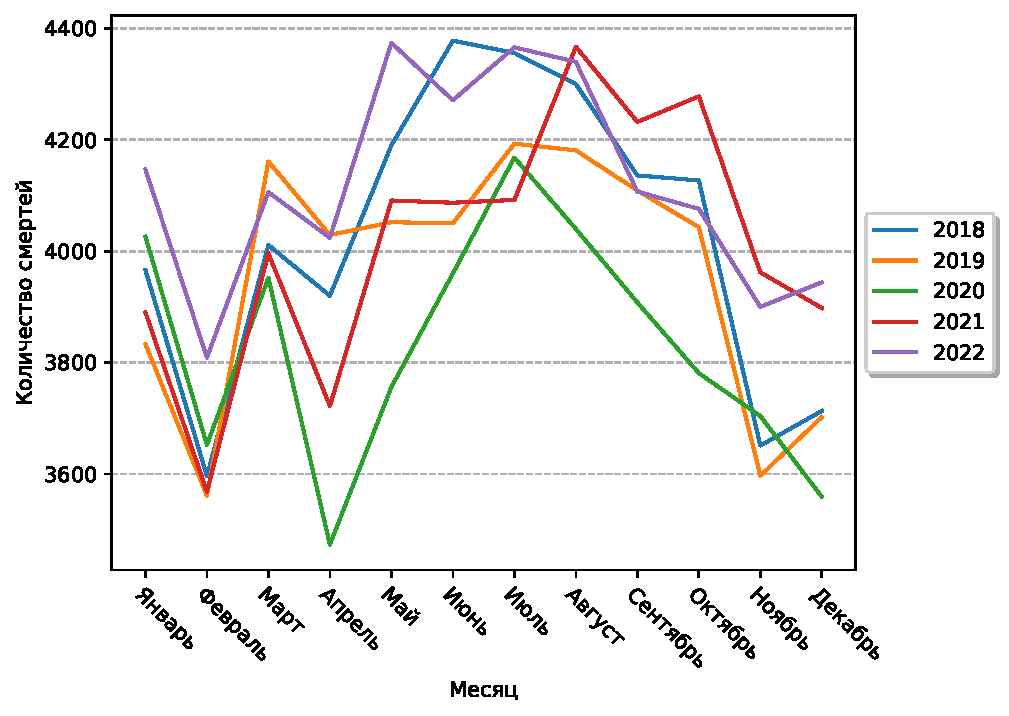
\includegraphics[width=0.9\textwidth]{inc/deathToMonth.pdf}
	\caption{ График количества смертей от суицида в определенные месяцы за 2018--2022 год. }\label{img:cdcsuicides}
\end{figure}

Признаки паттернов суицидального поведения человека по своей форме проявления могут быть \textit{явными} и \textit{неявными}. К явным признакам суицидального поведения относятся просьбы о помощи, в то время как к неявным~-- намеки на собственное состояние, депрессивные высказывания, изоляция от общества. Каждая форма проявления, как просьба о помощи, может выражаться:

\begin{itemize}
	\item аудиально~-- с использованием речевого аппарата, интонаций, музыкальных композиций;
	\item в текстовом виде~-- записка или сообщение;
	\item визуально~-- с использованием собственного имиджа, жестов, паттернов движений;
	\item социально~-- через изоляцию или конфликты с обществом;
	\item физиологически~-- затяжная депрессия, приводящая к суицидальным наклонностям, сказывается на состоянии организма человека.
\end{itemize}

В сети интернет наиболее доступными являются явные и неявные признаки, выражающиеся в текстовом виде, причем в качестве анализируемого материала могут использоваться как личные сообщения, так и предоставляемые широкому кругу лиц тексты с описанием жизненных ситуаций, собственного состояния или личных переживаний.

\subsection{Форматы хранения проявление поведения человека}

Для автоматизации анализа выражений форм проявления суицидального поведения человека и выявления патологий требуется определить формат хранения данных.

Результатом анализа \textit{аудиальных признаков} может быть наличие в словах человека депрессивных высказываний или интонаций пользователя в разговоре, умеющем суицидальный подтекст. Анализ аудио-сообщений подразумевает их расшифровку и сопоставление определенных высказываний с проявляемыми эмоциями. Далее под ``эмоциональной картой аудио-дорожки'' имеется в виду структура, в которой для определенных аудио-фрагментов сопоставлена одна из рассматриваемых эмоций пользователя. Данная структура может быть представлена как временные промежутки аудио-сообщения или как указатель на части расшифровки. 

Результатом анализа  \textit{текстовых сообщений} может быть наличие в сообщении каких-либо суицидальных признаков: употребление выражений, подразумевающих суицидальную тематику, слова с суицидальным подтекстом, прямые высказывания о желании совершить суицид.

Результатом анализа \textit{пространственно-временных признаков} может быть выявление подверженности жителей определенных регионов депрессии в связи с происходящими в них событиями или же соотнесение временных промежутков цикличным сезонам депрессии.

Результатом анализа \textit{визуальных признаков} может быть определение проявления суицидального поведение, попытки суицида, либо его совершение, а также определение депрессии по мимике в течение разговора. Анализ визуальных признаков подразумевает обработку видеозаписей с действиями человека.

\textit{Социальные признаки} могут выражаться как действия самого человека в социальной сфере или же информация, поступающая из социальной среды исследуемого индивидуума. Результатом анализа данных признаков может быть установление факта социальной изоляции, либо встревоженность окружения: родственников, друзей или знакомых. Анализ подразумевает мониторинг социальных связей человека или сбор данных о наблюдениях окружающих индивида людей.

Анализ \textit{физиологических признаков} может включать в себя либо диагностику депрессивного состояния, либо частотность присутствия исследуемого в стрессовых ситуациях, которые сопровождаются стадией истощения организма. \textit{Общий адаптационный синдром}~-- это сочетание стереотипных реакций, возникающих в организме в ответ на действие стрессоров и обеспечивающих ему устойчивость не только к стрессорному агенту, но и по отношению к другим болезнетворным факторам~\cite{stressAndPatology}. Определены три стадии общего адаптационного синдрома: тревоги, устойчивости и истощения. При длительном воздействии стрессора адаптивные механизмы, участвующие в поддержании резистентности, исчерпывают себя, и наступает стадия истощения организма. Данная стадия не является обязательной и стрессовая ситуация может быть окончена до ее наступления. Протекание реакции заключается в активизации эндокринной системы и обеднении коры надпочечников.~\cite{stressAndPatology}

Анализ \textit{биологических признаков} подразумевает под собой настройку чувствительности модели путем отнесения человека к известным группам риска. Согласно исследованиям в 2021 году констатировано 38 358 смертей в 2021 году и 39255 в 2022 году в результате суицида среди мужчин~\cite{suicideStats}. Среди женщин зафиксировано 9~825 смертей в 2021 году и 10~194 смертей в 2022 году~\cite{suicideStats}. Таким образом, по данной статистике мужчины совершают $\approx 80\%$ самоубийств, что говорит о том, что пол имеет важную роль в определении суицидального поведения индивида. Также, согласно исследованиям чаще всего суицид совершают люди возрастной группы 25~-44 лет и 45~-64 лет, в 2021 году зафиксировано, что они составили совместно для этих групп $\approx 65 \%$ всех самоубийств в США, а в 2022 году $\approx 66\%$~\cite{suicideStats}.


\subsection{Классификация сообщений в сети Интернет}

В настоящее время в сети Интернет большое количество событий, явлений и процессов описывается в относительно коротких текстовых сообщениях до 3 000 символов.
Их основными источниками являются сетевые новостные агентства.
Накопленные информационными службами массивы таких сообщений активно используются при наблюдении за обстановкой, состояниями объектов, общественным мнением.
Современное развитие сетевых СМИ, а также средств автоматического сбора текстовой информации сети Интернет позволяет информационным службам получать тысячи сообщений в день.
Так, только одно сетевое новостное агентство федерального уровня, как правило, выпускает несколько десятков сообщений в день, а роботизированные системы сбора сообщений позволяют обрабатывать сотни подобных источников.
Информационные потоки большой интенсивности и размерности делают невозможным ознакомление эксперта с каждым сообщением и вычленением его семантики.
Одним из решений данной проблемы является использование средств автоматической классификации текстовых сообщений, а необходимым условием эффективной работы подобным систем является применение алгоритма, обеспечивающего необходимое качество классификации. \cite{messageClassification}

Популяризация и развитие всемирной паутины и расширение глобальных компьютерных сетей, в том числе пополнение информационных баз данных, повлекло за собой наращивание текстовых ресурсов.
При интенсивном и постоянном возрастании объемов текстовой информации сложность поиска требуемых сведений среди огромного количества доступных текстов и сообщений значительно уменьшают ее ценность.
Классификация сообщений необходима для решения следующих задач \cite{classificationPromlems}:
\begin{itemize}
	\item обнаружение спама;
	\item разделение сайтов по тематическим каталогам;
	\item распознавание эмоциональной окраски текстов;
	\item автоматизация процесса исследования естественного языка;
	\item генерация текста;
	\item автоматическая обработка текста на естественном языке.
\end{itemize}

Существующие подходы к решению задач анализа текстов и обработки естественного языка включают в себя \cite{classificationPromlems}:

\begin{itemize}
	\item эмпирические методы, основанные на вероятностных моделях машинного обучения в области обработки естественного языка \cite{shit1};
	\item выявление психических заболеваний с помощью обработки естественного языка, выраженных в разнообразных текстовых данных, включая сообщения в социальных сетях \cite{shit2};
	\item статистика достоверности электронных медицинских карт и восстановления показателей из плохо читаемых сообщений при помощи методов анализа естественного языка \cite{shit3};
	\item взаимосвязь между эмоциями и настроениями клиентов, возникающими при взаимодействии с роботами в отелях с использованием методов анализа текста \cite{shit4};
	\item исследование тональности финансовой информации на английском языке при помощи метода анализа больших данных и нейронных сетей \cite{shit5};
	\item анализ настроений и эмоций для выявления стресса человека на основе сообщений и комментариев при помощи машинного обучения \cite{shit6}.
\end{itemize}

Задача определения тональности сообщений также может быть отнесена к задаче классификации сообщений, однако она не может решать более сложные проблемы, требующие изменения не только системы определения тональности. 
Зачастую при ее решении задействуют нейронные сети \cite{classificationPromlems}, либо различные методы машинного обучения \cite{presuicidalSignals}.
В качестве методов машинного обучения зачастую рассматриваются \cite{presuicidalSignals}:

\begin{itemize}
	\item Изоляционный лес;
	\item Локальный уровень выброса;
	\item Логистическая регрессия;
	\item OneClassSVM;
	\item Случайный лес;
	\item XGBoost \cite{boosting}.
\end{itemize}

Классификация сообщений необходима в организации социальных сетей для соблюдения порядка и своевременного обнаружения сообщений, разжигающих национальную рознь, призывающих к беспорядкам или оскорбляющих правительственную систему.
Также известно о наличии в некоторых социальных сетях и искусственного интеллекта, предназначенного для обнаружения людей с высоким суицидальным риском \cite{faceSuicide}, однако исходники не представляются, а все наработки являются объектами коммерческой тайны.


\subsection{Формализация задачи метода распознавания суицидальных паттернов поведения человека по текстовым сообщениям}

Метод распознавания суицидальных паттернов поведения человека по текстовым сообщениям включает в себя xранение и анализ сообщений пользователей. Для определения, является ли сообщение суицидальным, используется модель машинного обучения. В качестве обучающей выборки используется дополненный датасет размеченных сообщений из открытого доступа \cite{dataset}.

На рисунке \ref{img:idef0} представлена IDEF0 диаграмма нулевого уровня задачи определения наличия суицидальных паттернов в текстовом сообщении.

\begin{figure}[H]
	\centering
	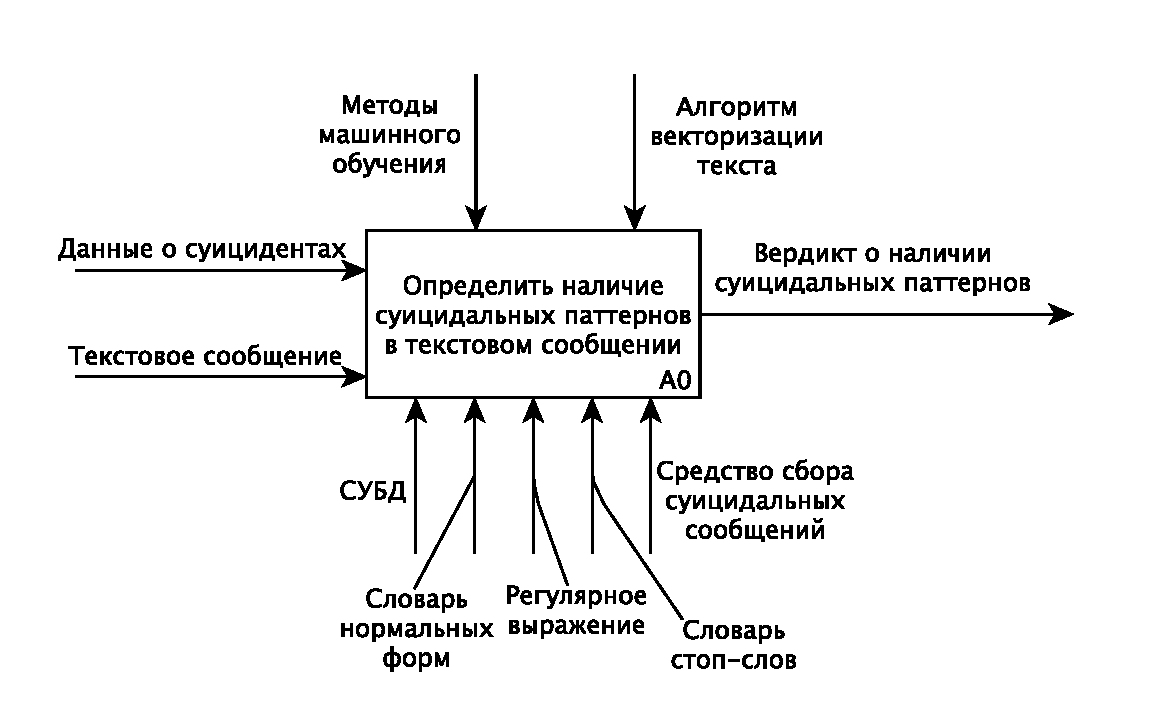
\includegraphics[width=\textwidth]{inc/A0.pdf}
	\caption{ IDEF0 диаграмма нулевого уровня. }
	\label{img:idef0}
\end{figure}


\subsubsection*{Вывод}

Были рассмотрены термины предметной области, включающие в себя понятия самоубийства и суицидального поведения. 
Представлен интегративный теоретический подход в суицидологии, описаны суицидальное поведение, внешние проявления суицидального поведения, пресуицид, парасуицид и постсуицид. 
Приведена информация об определении истинности суицидальных намерений, включившая в себя обстоятельства попытки и медицинские критерии. 

Описаны факторы повышенного суицидального риска и мероприятия и методики предотвращения самоубийств, включающие в себя суицидологическую диагностику, кризисную терапию и Телефон Доверия.
Представлена статистика совершения самоубийств.

С использованием классификации признаков паттернов суицидального поведения человека описаны форматы хранения проявления поведения человека, представленные в таблице~\ref{table:formats}. 
Были выделены аудиальные, текстовые, пространственно-временные, визуальные, физиологические и биологические признаки.
В рамках разрабатываемого метода анализируются лишь текстовые признаки.

\begin{sidewaystable}
\begin{table}[H]
	\begin{center}
		\caption{\label{table:formats} Форматы описания признаков и их методов обработки}
		\begin{tabular}{|p{4cm}|p{8cm}|p{12cm}|}
 			\hline
			Признаки & Данные & Методы обработки \\
 			\hline\hline
			\multirow{3}{*}{Аудиальные} & аудиофайл & распознавание речи, обработка и анализ текстовых сообщений, анализ характеристик голоса \\
			\cline{2-3}
			& текстовая расшифровка речи & обработка и анализ текстовых сообщений \\
			\cline{2-3}
			& эмоциональная карта,\newline{}аудиофайл / текстовая расшифровка & сопоставление эмоциональной карты смысловой нагрузке речи \\
 			\hline\hline
			\multirow{3}{*}{Текстовые} & текстовое сообщение & обработка и анализ текстовых сообщений с использованием методов машинного обучения \\
			\cline{2-3}
			& текстовое сообщение,\newline{}эмоциональная карта & уточнение входных данных модели с использованием эмоциональной карты \\
 			\hline\hline
			\multirow{2}{*}{\shortstack[l]{Пространственно-\\ временные}} & дата написания & соотнесения дат действий пользователя сезонности депрессии \\
			\cline{2-3}
			& место дислокации автора,\newline{}дата написания & соотнесение контекста происходящего в регионе пользователя его действиям  \\
			\hline\hline
			\multirow{3}{*}{Визуальные} & видеоряд действий пользователя & распознавание эмоций \\
			\cline{2-3}
			& видеоряд действий пользователя,\newline{}мониторинг контекста происходящего & анализ реакций индивидуума на внешние раздражители и жизненные ситуации \\
 			\hline\hline
			\multirow{3}{*}{Физиологические} & данные мониторинга уровня стресса & \multirow{3}{*}{\shortstack[l]{анализ состояния организма человека и его\\подверженности стрессам}} \\
			\cline{2-2}
			& данные мониторинга уровня кортизола в крови &  \\
			\cline{2-2}
			& данные мониторинга состояния здоровья человека &  \\
			\hline\hline
			\multirow{2}{*}{Биологические} & пол пользователя & уточнение входных данных модели с использованием пола пользователя \\
			\cline{2-3}
			& возраст пользователя & уточнение входных данных модели с использованием возрастной группы пользователя  \\
 			\hline
		\end{tabular}
	\end{center}
\end{table}
\end{sidewaystable}

\pagebreak